\title{Estimating Mutual Information from Average Classification Error}
\author{Charles Zheng and Yuval Benjamini}
\date{\today}

\documentclass[12pt]{article} 

% packages with special commands
\usepackage{amssymb, amsmath}
\usepackage{epsfig}
\usepackage{array}
\usepackage{ifthen}
\usepackage{color}
\usepackage{fancyhdr}
\usepackage{graphicx}
\usepackage{mathtools}
\usepackage{csquotes}
\definecolor{grey}{rgb}{0.5,0.5,0.5}

\begin{document}
\maketitle

\newcommand{\tr}{\text{tr}}
\newcommand{\E}{\textbf{E}}
\newcommand{\diag}{\text{diag}}
\newcommand{\argmax}{\text{argmax}}
\newcommand{\Cov}{\text{Cov}}
\newcommand{\Var}{\text{Var}}
\newcommand{\argmin}{\text{argmin}}
\newcommand{\Vol}{\text{Vol}}
\newcommand{\comm}[1]{}
\newcommand{\indep}{\rotatebox[origin=c]{90}{$\models$}}

\begin{abstract}
Multivariate pattern analyses approaches in neuroimaging are fundamentally concerned with investigating
the quantity and type of information processed by various regions of the human brain;
typically, estimates of classification accuracy are used to quantify information.
While a extensive and powerful library of methods can be applied to train and assess classifiers,
it is not always clear how to use the resulting measures of classification performance to draw scientific conclusions:
e.g. for the purpose of evaluating redundancy between brain regions.
An additional confound for interpreting classification performance is the dependence of the error rate on
the number and choice of distinct classes obtained for the classification task.
In contrast, mutual information is a quantity which is in principle defined independently of the experimental design,
and has ideal properties for comparative analyses.
One obstacle to wider use of mutual information is the difficulty of estimating mutual information in high-dimensional neuroimaging data.
%Nonparametric estimators have poor finite-sample performance, and parametric approaches require unrealistic assumptions such as multivariate Gaussianity.
%While one can obtain a lower bound using the mutual information of the confusion matrix, the lower bound obtained is usually quite poor.
We propose a new estimator of mutual information based on the concept of "average Bayes error."
By assuming that the classes obtained in the data are drawn randomly from a continuous population,
we find that the expected Bayes error converges to a function of the mutual information in a high-dimensional limit.
We demonstrate the utility of our approach in simulated and real-data examples.
\end{abstract}


\section{Introduction}

Many of the key questions motivating neuroimaging studies involve some concept of information:
which brain region processes sensory information?  how is information encoded in the form of memories?
To answer whether or not a particular brain region receives information about a given stimulus,
it suffices to demonstrate a systematic dependence between brain activity in that region and stimulus features;
this was the approach taken for studying single-cell recordings.
Moving beyond single-cell recordings, it becomes desirable to use methods which can quantify
the information encoded by populations of cells.

Following the seminal work by Haxby (2001), the dominant approach in this area,
known as ``multivariate pattern analysis'' (MVPA), is to quantify information in the form of classification error.
The classification approach contrasts with more traditional measures of information, such as mutual information and Fisher information.
For example, to demonstrate that a particular brain region responds to a certain type of sensory information,
one employs supervised learning to build a classifier which classifies the stimulus class from the brain activation in that region,
and tests the statistical hypothesis that the classifier has above-chance classification accuracy.
In principle, one could just as well test the statistical hypothesis that the Fisher information or mutual information between
the stimulus and the activation patterns is nonzero.  But in practice, the machine learning approach enjoys several advantages over
approaches based on estimating Fisher information or mutual information.
First, one does not need a parameterization of the stimulus space: this is highly relevant for studying complex stimuli such as faces.
Secondly, the machine learning approach does not require parametric model assumptions, unlike Fisher information.
Thirdly, the machine learning approach scales well with dimensionality of both the stimulus space and the response space.
In contrast, nonparametric methods for estimating mutual information scale extremely poorly with dimensionality of the response space.
Meanwhile, a major detractor for using classification error as a measure of information is that the classification accuracy depends on the particular choice of stimuli exemplars employed in the study and the number of partitions used to define the classes for the classification task.
The difficulty of the classification task depends on the number of classes defined: high classification accuracy can be achieved relatively easily by using a coarse partition of stimuli exemplars into classes.
In a meta-analysis on visual decoding, Coutanche et al (2016) quantified the strength of a classification study
using the formula
\[
\text{decoding strength} = \frac{\text{accuracy} - \text{chance}}{\text{chance}}.
\]
Such an approach may compensate for the differences in accuracy due purely to choice of number of classes defined;
however, no theory is provided to justify the formula.

In contrast, mutual information has ideal properties for the quantitatively 
comparing information between different studies, or between different brain regions, subjects, featurization models, or modalities.
Not only is the mutual information defined independently of the arbitrary definition of stimulus classes (albeit still dependent on an
implied distribution over stimuli), it is even meaningful to discuss the difference between the mutual information measured for one system
and the mutual information for a second system.
Due to these appealing properties, as well as the success of information theoretic approaches in more traditional neuroscience studies,
mutual information has been frequently proposed for application in neuroimaging studies (Quiroga 2009).
However, since nonparametric approaches for estimating mutual information are unusably inaccurate for typical high-dimensional data sets,
alternative approaches must be employed.  One can tractably estimate mutual information by assuming a multivariate Gaussian model:
however, this approach essentially assumes a linear relationship between the input and output, and hence fails to quantify nonlinear dependencies.
Alternatively, one can obtain a lower bound on the mutual information from the confusion matrix of the classifier.
This is the most popular approach for estimating mutual information in neuroimaging studies, but suffers from known shortcomings
(Gastpar 2010, Quiroga 2009).

The idea of linking classification performance to mutual information is not new: 
after all, Shannon's original motivation was to characterize the minimum achievable error probability
of a noisy communication channel.  More explicitly, Fano's inequality provides a
lower bound on mutual information in relation to the optimal prediction error, or Bayes error.
Fano's inequality can be further refined to obtain a tighter lower bound on mutual information (Tebbe and Dwyer 1968.)

In practice, the idea of deriving estimates of mutual information from classification performance occupies an advantageous middle ground
between the two extremes of nonparametric and parametric approaches for estimating mutual information.
In neuroimaging data, we lack prior knowledge for specifying parametric models, and the data is too high-dimensional for nonparametric approaches,
but we have a sufficient idea of the general ``structure'' in the data to achieve above-chance classification rates.

However, there are several practical issues for estimating mutual information from classification accuracy. 
One, the achievable classification accuracy depends on the amount of data available for training.
The test error is a unbiased estimate of the true error rate of the classifier on new data (called generalization error);
but in turn, the generalization error can only be meaningfully interpreted as a lower bound on the error rate of the ideal classfier,
or Bayes error.  Secondly, even if one could obtain the Bayes error, the Bayes error itself depends on the choices made by the experimenter
in regards to the stimuli exemplar chosen in the experiment, and the decision of how to partition those exemplars in the classification task.
For example, Nishimoto et al classified segments of a movie clips based on activation patterns, but the definition of the classification task,
and the achievable classification performance, depends not only on the particular move clips used in the experiment, but also
the choice of time interval used to define discrete classes: defining each class to be a 1sec segment of movie results in more distinct classes
and lower classification accuracy than defining each class to be a 4sec segment of movie.
The Bayes error, and any estimate of mutual information based on the Bayes error, would therefore be necessarily dependent on the experimental parameters.

In principle, the first issue can be overcome by having sufficiently many observations: but a practical issue is that an astronomical amount
of data might be needed to learn the optimal classification rule.  A more efficient approach would be to estimate the Bayes error from
the classification performance.  Since the Bayes error is the large-sample limit of the achieved classification error, a promising approach is
to perform classification using differently sized subsamples of the training data, producing a plot of classification error versus sample size--a ``learning curve.''
One can then extrapolate the learning curve to estimate the Bayes error (Cortes et al. 1994.)
However, much work remains to develop rigorous methodology for estimating Bayes error, and so we leave this first issue for future work.

The starting point for our methodology is a proposal for overcoming the second issue: the non-uniqueness of the Bayes error.
We define a notion of $K$-class \emph{average Bayes error} which is uniquely defined for any given stimulus distribution and stochastic mapping from stimulus to response.  The $K$-class average Bayes error is simply the expectation of the Bayes error when $K$ stimuli exemplars are drawn i.i.d. from the stimulus distribution, and treated as distinct classes.  Hence the average Bayes error can in principle be estimated if the appropriate randomization is employed
for designing the experiment.

While the $K$-class average Bayes error is defined independently of the particular choice of stimuli,
the quantity still depends on the choice of number of classes, $K$.
In comparison, the mutual information provides a quantification of information which does not depend on $K$,
allowing more flexible comparisons and easier interpretation.
Hence our main theoretical contribution is the derivation of an asymptotic relationship between the $K$-class average Bayes error
and the mutual information, which in practice means that any estimate of the $K$-class Bayes error can be converted into an estimate of mutual information;
and the resulting estimator of mutual information should be asymptotically independent of the choice of number of classes $K$.

\section{Average Bayes Error}

The following simplified model captures the essence of many neuroimaging studies.
Let $\mathcal{X}$ be a space of stimuli, represented by $q$-dimensional vectors.
In the design stage of the experiment, a set of stimuli exemplars $\{x_1,\hdots, x_k\}$ are selected,
and then one specifies a $T$-length sequence of stimuli $( x_{i_1},\hdots, x_{i_n} )$ to be presented to the subject.
In the execution of the experiment, an activation pattern, or \emph{response} $y_t$ is obtained for each of the stimuli presentations $x_{i_t}$.
Generally $y_t$ is a $p$-dimensional vector, representing activity levels of $p$ disjoint brain regions.
To simplify, assume that each of the $k$ stimuli is presented a total of $r$ times in the sequence;
further assume that the responses to each stimulus presentation are conditionally independent, hence the ordering of the sequence does not matter.
Henceforth we can let $y_i^j$ denote the response to the $j$th presentation of the stimulus $x_i$.

We now restate the model in application-independent terms.  Let $\mathcal{X} \subset \mathbb{R}^q$ and $\mathcal{Y} \subset \mathbb{R}^p$;
let $p(x)$ be a probability density on $\mathcal{X}$.  For every $x \in \mathcal{X}$, let $p_x(y)$ be a probability density on $\mathcal{Y}$.
Define the joint density
\[
p(x, y) = p(x) p_x(y)
\]
so that $p_x(y)$ can also be written $p(y|x)$.
Take a  subset $\{x_1,\hdots, x_k\} \subset \mathcal{X}$.  Let $Y_i^j$ be a random vector distributed according to density $p_{x_i}(y)$;
and let $Y_i^j$ be conditionally independent given $\{x_1,\hdots, x_k\}$ for $i = 1,\hdots, k$ and $j = 1, \hdots, r.$
 
In MVPA, one carries out a classification task to assess whether $y$ contains information about $x$.
Formally, a classification rule is any (possibly stochastic) mapping $f: \mathcal{Y} \to \{1,\hdots, k\}$.
The \emph{generalization error} of the classification rule is
\[
e_{gen}(f) = \frac{1}{k} \sum_{i=1}^k\Pr[f(Y) \neq i | X = x_i].
\]
A trivial classification rule which outputs the result of a $k$-sided die roll for all inputs $y$ would achieve a generalization error of $e_{gen} = \frac{1}{k}$.
Conversely, even a single counterexample with $e_{gen} < \frac{1}{k}$ is indicative that $y$ contains nonzero information about $x$.
Hence, in order to demonstrate that $y$ is informative of $x$, one tests the null hypothesis
\[
H_0: e_{gen}(f) = \frac{1}{k}.
\]
Rejecting the null hypothesis for a given classification rule $f$ can be taken as evidence that $y$ is informative of $x$.
In the discussion thus far, ``information'' refers to an informal, intuitive notion, but it is also possible to formally establish
that violation of the null hypothesis implies nonzero mutual information $I(X; Y)$.



The classifier is a functional which maps a set of observations to a classification rule,
\[
\mathcal{F}: \{(x_1,y_1),\hdots, (x_m, y_m)\} \mapsto f(\cdot);
\]
informally, a classifier is an algorithm which ``learns'' a classification rule from data.
For a valid test of $H_0$, 
either the data-splitting approach or the cross-validation approach can be used.
In the data-splitting approach, one creates a \emph{training set} consisting of $r_1$ repeats per class,
\[
\{(x_1, y_1^1),\hdots, (x_1,y_1^{r_1}), \hdots, (x_m, y_m^1),\hdots, (x_m,y_m^{r_1})\}
\]
and a \emph{test set} consisting of the remaining $r_2 = r - r_1$ repeats.
\[
\{(x_1, y_1^{r_1 + 1}),\hdots, (x_1,y_1^{r}), \hdots, (x_m, y_m^{r_1 + 1}),\hdots, (x_m,y_m^{r_1})\}.
\]
In the cross-validation approach, one applies the data-splitting approach multiple times, with different training and test partitions, and aggregates the results.
We further discuss the cross-validation approach in section X.

In the data-splitting approach, one obtains the classification rule $f$ by applying the classifier to the training data,
\[
f = \mathcal{F}(\{(x_1, y_1^1),\hdots, (x_1,y_1^{r_1}), \hdots, (x_m, y_m^1),\hdots, (x_m,y_m^{r_1})\})
\]
The test statistic of interest is the test error,
defined as
\[
e_{test} = \frac{1}{k r_2} \sum_{i=1}^k \sum_{j = r_1 + 1}^r \text{I}(f(y_i^j) \neq i).
\]
Due to the conditional independence of the training set and test set, $e_{test}$ is an unbiased estimate of $e_{gen}$.
Hence various approaches can be used to obtain a threshold $c_\alpha$
such that $\Pr[e_{test} < c_\alpha] \leq \alpha$ holds (approximately) under the null hypothesis.
To name a few, one can employ permutation tests, tests based on a universal variance bound, or the generalized likelihood ratio test.
Regardless of the procedure used to derive the threshold $c_\alpha$, The hypothesis $H_0$ is rejected at level $\alpha$ if $e_{test} < c_\alpha$.

While tests of the generalization error suffice to establish the presence of information,
the generalization error is less satisfactory as a measure of the information between $X$ and $Y$,
since the $e_{gen}$ depends on the classification rule $f$ obtained, and hence, varies randomly depending on the sampling of the data.
For most reasonable classifiers, the generalization error decreases as the number of training observations increases.
Therefore, the sample size is an additional confounding factor for interpreting the generalization error.

A more ideal measure of information, still related to the classification, is the Bayes error, which is simply the \emph{optimal} generalization error
\[
e_{Bayes} = \min_f e_{gen}(f).
\]
Due to Bayes' theorem, the optimal classification rule $f^*$ which achieves the Bayes error can be given explicitly:
it is the maximum a posteriori (MAP) rule
\[
f^*(y) = \argmax_{i=1}^k\ p(y|x_i).
\]

Estimating $e_{Bayes}$ is much more difficult in practice than estimating $e_{gen}$;
however, nonparametric estimators of $e_{Bayes}$ have been proposed in the literature.
Cover (1969) first noted that the leave-one-out error of 1-nearest neighbor, $e_{1nn}$,
asymptotically bounds the Bayes error in the sense that
\[
\frac{1}{2}\E[e_{1nn}] \leq e_{Bayes} \leq \E[e_{1nn}].
\]
Later, Fukunaga and Kessel (1971) and Fralick and Scott (1971) both proposed a consistent estimator of $e_{Bayes}$
using the test error from kernel density estimation-based classifiers.
Fukunaga and Hostetler 1975 improved on the density estimation approach by estimating the generalization error directly,
rather than using empirical test error (hence reducing variance.)

Nevertheless, the convergence rates of nonparametric methods of Bayes risk estimation are too slow to provide much assurance
for their use in high-dimensional problems.  On the other hand, the empirical success of supervised learning approaches seems
to justify a certain optimism that at least one of the popular black-box methods (random forests, neural networks, kernel SVM)
can come close to the Bayes error rate within realistic sample sizes.  Methods such as random forests and neural networks
are known to have \emph{universal approximation} properties that guarantee consistent recovery of the classification rule,
given that the model complexity is scaled at an appropriate rate as the sample size increases; but methods such as kernel SVM
have much more restrictive function classes and therefore have no guarantee of being able to recover the Bayes error.
Yet, it is seen in many learning tasks that the test error is very similar for very different classification methods, 
some universal and some non-universal, suggesting that the true signal lies in a low-complexity function class which can
be adequately approximated using a variety of methods.  Empirical evidence for these phenomenon are collected in studies
on the learning curves of classifers, beginning with Cortes 1994, and applied to specific applications by Figueroa et al. 2012, Beleites et al. 2013.
We leave further discussion of Bayes error estimation for future work; in the theoretical portion of the current paper,
we will simply leave unspecified the method used to estimate Bayes error, and in our simulation and real data examples,
we will use an ad hoc approach for estimating Bayes error from test error for the purpose of demonstrating our method.

As we pointed out in the introduction, the quantity $e_{Bayes}$ is not a parameter of the joint distribution $p(x, y)$,
but rather depends on the specific exemplars $x_1,\hdots, x_k$ selected;
hence, one may write $e_{Bayes}(x_1,\hdots, x_k)$ to emphasize this dependence.
In many studies, the end goal is to make some inference about the joint distribution $p(x, y)$, such as the mutual information $I(X; Y)$.
However, an estimate of $e_{Bayes}$ cannot possibly be sufficient as a basis for inference about $p(x, y)$ because
there is no direct link between $e_{Bayes}$ and $p(x)$, given that we made no assumption on how $x_1,\hdots, x_k$ were obtained.
This motivates definition of the \emph{average} Bayes error,
\[
e_{ABE} = \E[e_{Bayes}(X_1,\hdots, X_k)],
\]
where $X_1,\hdots, X_K$ are drawn i.i.d. from $p(x)$.
The $k$-class average Bayes error is uniquely defined for any joint distribution $p(x, y)$,
and supposing that an unbiased estimator for Bayes error exists, $\hat{e}_{Bayes}$,
then $\hat{e}_{Bayes}$ will also be unbiased for $e_{ABE}$ supposing that the experimental design randomized the selection of $X_1,\hdots, X_k$
by drawing the vectors independently from $p(x)$.

In the following section we investigate the relationship between $e_{ABE}$ and the mutual information $I(X; Y)$.

\section{Asymptotic Theory}

Our goal in this section is to establish a relationship between the mutual information $I(X; Y)$ and the $k$-class average Bayes error, $e_{ABE}$.
In short, we will show that for some function $\pi_k$ (which depends on $k$), 
\[
e_{ABE} \approx \pi_k(\sqrt{2 I(X; Y)})
\]
and that this approximation becomes accurate under a limit where $I(X; Y)$ is small relative to the dimensionality of $X$,
and under the condition that the components of $X$ are approximately independent.  Formal conditions are given in the proof statement.

First, let us rewrite $e_{ABE}$ in terms of the density function.  Recall that the Bayes rule is
\[
e_{Bayes}(x_1,\hdots, x_k) = \frac{1}{k}\sum_{i=1}^k \Pr[\hat{X}(Y) \neq x_i| X = x_i].
\]
In turn, the Bayes classification rule is given in terms of the conditional density:
\[
\hat{X}(y) = \argmax_{x \in \{x_1,\hdots, x_k\}} p(y|x).
\]
Therefore, we obtain
\[
e_{Bayes}(x_1,\hdots, x_k) = \frac{1}{k}\sum_{i=1}^k \Pr[p(Y|x_i) \leq \max_{j \neq i} p(Y|x_j)| X = x_i].
\]
In turn the average Bayes error can be written as
\begin{align}
e_{ABE} &= \E[e_{Bayes}(X_1,\hdots, X_k)]
\\&= \frac{1}{k}\sum_{i=1}^k \E[\Pr[p(Y|x_i) \leq \max_{j \neq i} p(Y|x_j)| X = x_i]]
\\&= \E[\Pr[p(Y|x_1) \leq \max_{j \neq 1} p(Y|x_j)| X = x_1]]
\\&= \Pr[p(Y|X_1) \leq \max_{j \neq 1} p(Y|X_j)| X = X_1].
\end{align}

Defining $Z_i = \log p(Y|X_i) - \log p(Y|X_1)$, where $Y \sim p(y|X_1)$.
The we obtain
\[
e_{ABE} = \Pr[Z_1 < \max_{j > 1} Z_i].
\]

Our proof uses the assumption that $Z_1,\hdots, Z_k$ are asymptotically multivariate normal.
To see why this might be justified, suppose that $X$ and $Y$ have the same dimensionality $d$, and that
joint density factorizes as
\[
p(x_j, y) = \prod_{i=1}^d p_i(x_{j, i}, y_i)
\]
where $x_{j, i}, y_i$ are the components of $x_j$ and $y$.
Then,
\[
Z_i = \sum_{m=1}^d \log p_m(y_m | x_{m, i}) - \log p_m(y_m | x_{m, 1})
\]
where $x_{i, j}$ is the $i$th component of $x_j$.
The $d$ terms $\log p_m(y_m | x_{m, i}) - \log p_m(y_m | x_{m, 1})$ are independent across the indices $m$,
but dependent between the $i = 1,\hdots, k$.
Therefore, the multivariate central limit theorem can be applied to conclude that the vector
$(Z_1,\hdots, Z_k)$ can be scaled to converge to a multivariate normal distribution.
Now, since the average Bayes error $e_{ABE}$ is a continuous functional of the joint distribution $p(x, y)$,
it follows that $e_{ABE}$ converges to a functional of the limiting mean and covariance of $(Z_1,\hdots, Z_k)$, assuming
that the limits exist.
In our theorem, we assume a specific regime where these limits exist as a consequence.
While the componentwise independence condition is not a realistic assumption,
the key property of multivariate normality of $(Z_1,\hdots, Z_k)$ holds under more general conditions, and appears reasonable in practice.

The second component of our theorem is to manipulate the expression of the mutual information $I(X; Y)$.
The differential mutual information is defined as
\[
I(X; Y) = \int p(x, y) \log \frac{p(x, y)}{p(x) p(y)} dx dy.
\]
The key manipulation we employ is to approximate the logarithmic term by the Taylor expansion
\[
\log \frac{p(x, y)}{p(x) p(y)} \approx \frac{p(x, y) - p(x) p(y)}{p(x) p(y)} - \left(\frac{p(x, y) - p(x) p(y)}{p(x) p(y)}\right)^2 + \hdots.
\]
The approximation is accurate if $I(X; Y)$ is small--or rather, small relative to the dimensionality within the asymptotic sequence.
We state the theorem for the regime where $I(X; Y)$ is fixed, while the dimensionality of $X$ increases.

The function $\pi_k$ is given by
\[
\pi_k(c) = 1 - \int_{\mathbb{R}} \phi(z - c)  \Phi(z)^{k-1} dz.
\]
Figure \ref{fig:pi} displays the plot of $\pi_k$ for several values of $k$.
For all values of $k$, $\pi_k(\mu)$ is monotonically decreasing in $\mu$, and tends to zero as $\mu \to \infty$.
This should not be surprising, because if $I(X; Y)$ is large, then the average Bayes error should be small.
Another fact, which can be verified through a simple calculation, is that 
\[
\pi_k(0) = 1 - \frac{1}{k}.
\]
This should also not be surprising, since if $I(X; Y) = 0$, then it should not be possible to
obtain a classification rule which is better than guessing at random, which is only correct with probability $1/k$.
\begin{figure}
\centering
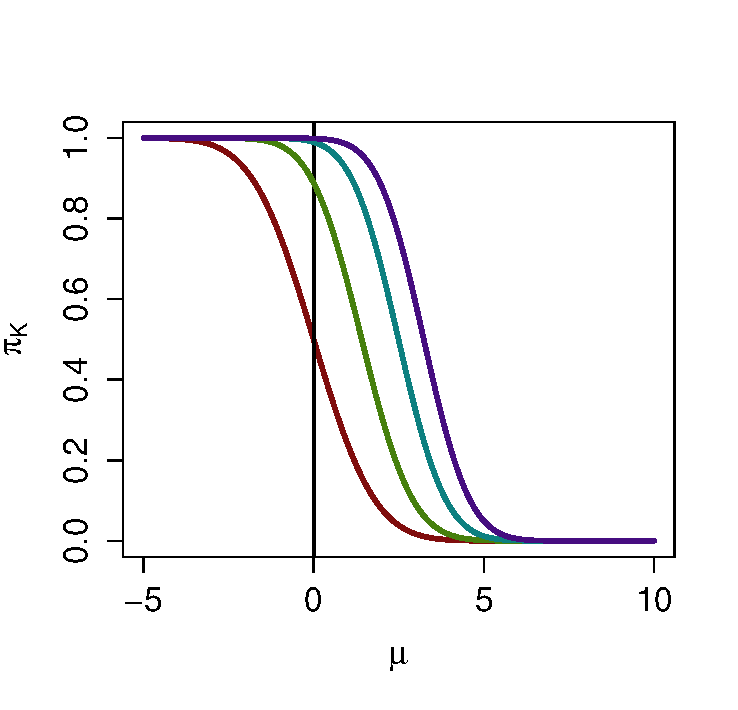
\includegraphics[scale = 0.5, clip=true, trim=0 0.2in 0 0.5in]{../info_theory_sims/illus_piK.pdf}
\caption{The function $pi_k(\mu)$, for $k = \{2, 9, 99, 999\}$ (left to right) \label{fig:pi}}
\end{figure}


\subsection{Technical section}

We formally state the assumptions and theorem in this section.  The less technically inclined reader may skip the section in order to continue to the proposed methodology for estimating mutual information, and results. [Note: slightly different notation in this section: we will make the notation consistent with the rest of the paper before submission.]

The asymptotic regime we consider is one where the dimension of $X$ goes to infinity.
This means that we have to consider a sequence of joint distributions $(X^{[d]}, Y^{[d]})$ indexed by the dimension $d$.

Fix integer $K \geq 2$.  Let $p^{[d]}(x,y)$ be a sequence of
probability density functions, where $x$ is of dimension $p^{[d]}$ and
$y$ is of dimension $q^{[d]}$.  Let $p^{[d]}(x)$ and $p^{[d]}(y)$
denote the marginal densities, and let
\[
p^{[d]}(y|x) = p^{[d]}(x, y)/p^{[d]}(y).\]
 Let $(X^{([d], i)}, Y^{([d], i)})$ be
iid random variates from $p^{[d]}(x, y)$ for $i = 0, \hdots, K-1$; we will supress the
superscripts $[d]$ and/or $(i)$ when convenient.  Recall the definitions of
entropy,
\[
H(X) = -\int p(x) \log p(x) dx,
\]
and mutual information
\[
I(X; Y) = \int p(x, y) \log \frac{p(x, y)}{p(x)p(y)} dx dy.
\]
Furthermore, define the $K$-class average Bayes error as
\[
\text{ABE}_K = \Pr[p(Y^{(0)}|X^{(0)}) < \max_{i = 1}^{K-1} p(Y^{(0)}|X^{(i)})].
\]
Define
\[
u^{[d]}(x, y) = \log p^{[d]}(x, y) - \log p^{[d]}(x) - \log p^{[d]}(y),
\]
and define
\[
\ell_{ij}^{[d]} = \log p(y^{(i)}|x^{(j)}).
\]

We will need the following lemma:

\textbf{Lemma 1. }
\emph{
Suppose $(Z_*, Z_1, \hdots, Z_{K-1})$ are jointly multivariate normal, with 
$\E[Z_* - Z_1]= \alpha$, 
$\Var(Z_*) = \beta$, 
$\Cov(Z_*, Z_i) = \gamma$, 
$\Var(Z_i)= \delta$, and $\Cov(Z_i, Z_j) = \epsilon$ for all $i, j = 1, \hdots,
K-1$, such that $\beta + \epsilon - 2\gamma > 0$.  Then, letting
\[
\mu = \frac{\E[Z_* - Z_i]}{\sqrt{\frac{1}{2}\Var(Z_i - Z_j)}} = \frac{\alpha}{\sqrt{\delta - \epsilon}},
\]
\[
\nu^2 = \frac{\Cov(Z_* -Z_i, Z_* - Z_j)}{\frac{1}{2}\Var(Z_i - Z_j)} = \frac{\beta + \epsilon - 2\gamma}{\delta - \epsilon},
\]
we have
\begin{align*}
\Pr[Z_* < \max_{i=1}^{K-1} Z_i] &= \Pr[W < M_{K-1}]
\\&= 1 - \int \frac{1}{\sqrt{2\pi\nu^2}} e^{-\frac{(w-\mu)^2}{2\nu^2}} \Phi(w)^{K-1} dw,
\end{align*}
where $W \sim N(\mu, \nu^2)$ and $M_{K-1}$ is the maximum of $K-1$
independent standard normal variates, which are independent of $W$.
}

\textbf{Proof.}
We can construct independent normal variates $G_0$, $G_1,\hdots, G_{K-1}$
such that
\[
G_0 \sim N(0, \beta + \epsilon - 2 \gamma)
\]
\[
G_i \sim N(0, \delta - \epsilon)
\]
such that
\[
Z_* - Z_i = \alpha + G_0 + G_i.
\]
Hence
\begin{align*}
\Pr[Z_* < \max_{i=1}^{K-1} Z_i] &= \Pr[\min_i Z_* - Z_i < 0].
\\&= \Pr[\min_{i=1}^{K-1} G_0 + G_i + \alpha < 0]
\\&= \Pr[\min_{i=1}^{K-1} G_i < -\alpha - G_0]
\\&= \Pr[\min_{i=1}^{K-1} \frac{G_i}{\sqrt{\delta - \epsilon}} < -\frac{\alpha - G_0}{\sqrt{\delta - \epsilon}}].
\end{align*}
Since $\frac{G_i}{\sqrt{\delta - \epsilon}}$ are iid standard normal variates, and since
$-\frac{\alpha - G_0}{\sqrt{\delta - \epsilon}} \sim N(\mu,\nu^2)$ for $\mu$ and $\nu^2$ given in the statement of the Lemma, the proof is completed via a straightforward computation.  $\Box$


We now give the theorem and its proof.

\textbf{Theorem 1.} Let $p^{[d]}(x, y)$ be a sequence of joint densities
for $d = 1,2,\hdots$ as given above.  Further assume that
\begin{itemize}
\item[A1.] $\lim_{d \to \infty} I(X^{[d]}; Y^{[d]}) = \iota < \infty.$
\item[A2.] There exists a sequence of scaling constants $a_{ij}^{[d]}$
and $b_{ij}^{[d]}$ such that the random vector $(a_{ij}\ell_{ij}^{[d]} +
b_{ij}^{[d]})_{i, j = 1,\hdots, K}$ converges in distribution to a
multivariate normal distribution.
\item[A3.] There exists a sequence of scaling constants $a^{[d]}$, $b^{[d]}$ such that
\[
a^{[d]}u(X^{(1)}, Y^{(2)}) + b^{[d]}
\]
converges in distribution to a univariate normal distribution.
\item[A4.] For all $i \neq k$,
\[\lim_{d \to \infty}\Cov[u(X^{(i)}, Y^{(j)}), u(X^{(k)}, Y^{(j)})] = 0.\]
\end{itemize}
Then for $\text{ABE}_K$ as defined above, we have
\[
\lim_{d \to \infty} \text{ABE}_{K} = \pi_K(\sqrt{2 \iota})
\]
where
\[
\pi_K(c) = 1 - \int_{\mathbb{R}} \phi(z - c)  \Phi(z)^{K-1} dz
\]
where $\phi$ and $\Phi$ are the standard normal density function and
cumulative distribution function, respectively.

\textbf{Proof.}

For $i = 1,\hdots, K-1$, define
\[
Z_i = \log p(Y^{(0)}|X^{(i)}) - \log p(Y^{(0)}|X^{(0)}).
\]
Then, we claim that $\vec{Z} = (Z_1,\hdots, Z_{K-1})$ converges in distribution to
\[
\vec{Z} \sim N\left(-2\iota, 
\begin{bmatrix}
4\iota & 2\iota & \cdots & 2\iota\\
2\iota & 4\iota & \cdots & 2\iota\\
\vdots & \vdots & \ddots & \vdots\\
2\iota & 2\iota & \cdots & 4\iota
\end{bmatrix}
\right).
\]
Combining the claim with the lemma (stated below this proof) yields the
desired result.

To prove the claim, it suffices to derive the limiting moments
\[\E[Z_i] \to -2\iota,\]
\[\Cov[Z_i] \to 4\iota,\]
\[\Cov[Z_i, Z_j] \to 2\iota,\]
for $i \neq j$,
since then assumption A2 implies the existence of a multivariate normal
limiting distribution with the given moments.

Before deriving the limiting moments, note the following identities.
Let $X' = X^{(1)}$ and $Y = Y^{(0)}$.
\[
\E[e^{u(X', Y)}] = \int p(x) p(y) e^{u(x, y)} dx dy = \int p(x, y) dx dy = 1.
\]
Therefore, from assumption A3 and the formula for gaussian exponential
moments, we have
\[
\lim_{d \to \infty} \E[u(X', Y)]-\frac{1}{2}\Var[u(X', Y)] = 0.
\]
Let $\sigma^2 = \lim_{d \to \infty} \Var[u(X', Y)]$.
Meanwhile, by applying assumption A2,
\begin{align*}
\lim_{d \to \infty} I(X; Y) &= \lim_{d \to \infty} \int p(x, y) u(x, y) dx dy 
= \lim_{d \to \infty} \int p(x) p(y) e^{u(x, y)} u(x, y) dx dy
\\&= \lim_{d \to \infty}  \E[e^{u(X, Y')}u(X, Y')]
\\&= \int_{\mathbb{R}} e^z z \frac{1}{\sqrt{2\pi \sigma^2}} 
e^{-\frac{(z + \sigma^2/2)^2}{2\sigma^2}} \text{ (applying A2)}
\\&= \int_{\mathbb{R}} z \frac{1}{\sqrt{2\pi \sigma^2}} 
e^{-\frac{(z - \sigma^2/2)^2}{2\sigma^2}}
\\&= \frac{1}{2}\sigma^2.
\end{align*}
Therefore,
\[
\sigma^2 = 2\iota,
\]
and
\[
\lim_{d \to \infty} \E[u(X', Y)] = -\iota.
\]
Once again by applying A2, we get
\begin{align*}
\lim_{d \to \infty} \Var[u(X, Y)] 
&= \lim_{d \to \infty} \int (u(x, y) - \iota)^2 p(x, y) dx dy
\\&= \lim_{d \to \infty} \int (u(x, y) - \iota)^2 e^{u(x, y)} p(x) p(y) dx dy
\\&= \lim_{d \to \infty} \E[(u(X', Y) - \iota)^2 e^{u(X', Y)}] 
\\&= \int (z - \iota)^2 e^z \frac{1}{\sqrt{4\pi\iota}} e^{-\frac{(z+\iota)^2}{4\iota}} dz \text{ (applying A2)}
\\&= \int (z - \iota)^2 \frac{1}{\sqrt{4\pi\iota}} e^{-\frac{(z-\iota)^2}{4\iota}} dz
\\&= 2\iota.
\end{align*}


We now proceed to derive the limiting moments.
We have
\begin{align*}
\lim_{d \to \infty} \E[Z] 
&= \lim_{d \to \infty} \E[ \log p(Y|X') - \log p(Y|X)]
\\&= \lim_{d \to \infty} \E[ u(X', Y) - u(X, Y) ] = -2\iota.
\end{align*}
Also,
\begin{align*}
\lim_{d \to \infty} \Var[Z]
 &= \lim_{d \to \infty} \Var[ u(X', Y) - u(X, Y) ]
\\&= \lim_{d \to \infty} \Var[ u(X', Y)] +\Var[ u(X, Y) ]\text{ (using assumption A4) }
\\&= 4\iota,
\end{align*}
and similarly
\begin{align*}
\lim_{d \to \infty} \Cov[Z_i, Z_j]
&= \lim_{d \to \infty} \Var[ u(X, Y)]\text{ (using assumption A4) }
\\&= 2\iota.
\end{align*}
This concludes the proof. $\Box$.

Assumptions A1-A4 are satisfied in a variety of natural models.
One example is a multivariate Gaussian model where
\[
X \sim N(0, \Sigma_d)
\]
\[
E \sim N(0, \Sigma_e)
\]
\[
Y = X + E
\]
where $\Sigma_d$ and $\Sigma_e$ are $d \times d$ covariance matrices, and where $X$ and $E$ are independent.  Then, if $d \Sigma_d$ and $\Sigma_e$ have limiting spectra $H$ and $G$ respectively,
the joint densities $p(x, y)$ for $d = 1,\hdots, $ satisfy assumptions A1 - A4.

We can also construct a family of densities satisfying A1 - A4,
which we call an \emph{exponential family sequence model} since each joint distribution in the sequence
is a member of an exponential family.
A given exponential family sequence model is specified by choice of a base carrier function $b(x, y)$ and base sufficient statistic $t(x, y)$, with the property that carrier function factorizes as
\[
b(x, y) = b_x(x) b_y(y)
\]
for marginal densities $b_x$ and $b_y$.
Note that the dimensions of $x$ and $y$ in the base carrier function are arbitrary;
let $p$ denote the dimension of $x$ and $q$ the dimension of $y$ for the base carrier function.
Next, one specifies a sequence of scalar parameters $\kappa_1, \kappa_2,\hdots$ such that
\[
\lim_{d \to \infty} d \kappa_d = c < \infty.
\]
for some constant $c$.
For the $d$th element of the sequence, $X^{[d]}$ is a $pd$-dimensional vector,
which can be partitioned into blocks
\[
X^{[d]} = (X_1^{[d]},\hdots, X_d^{[d]})
\]
where each $X_i^{[d]}$ is $p$-dimensional.  Similarly, $Y^{[d]}$ is partitioned into $Y_i^{[d]}$ for $i = 1,\hdots, d$.
The density of $(X^{[d]}, Y^{[d]})$ is given by
\[
p^{[d]}(x^{[d]}, y^{[d]}) = Z_d^{-1} \left(\prod_{i=1}^d b(x_i^{[d]}, y_i^{[d]}) \right) 
\exp\left[\kappa_d \sum_{i=1}^d t(x_i^{[d]}, y_i^{[d]}) \right],
\]
where $Z_d$ is a normalizing constant.
Hence $p^{[d]}$ can be recognized as the member of an exponential family with carrier measure
\[
\left(\prod_{i=1}^d b(x_i^{[d]}, y_i^{[d]}) \right)
\]
and sufficient statistic
\[
\sum_{i=1}^d t(x_i^{[d]}, y_i^{[d]}).
\]

One example of such an exponential family sequence model is a multivariate Gaussian model with limiting spectra $H = \delta_1$ and $G = \delta_1$, but scaled so that the marginal variance of the components of $X$ and $Y$ are equal to one.  This corresponds to a exponential family sequence model with
\[
b_x(x) = b_y(x) = \frac{1}{\sqrt{2\pi}} e^{-x^2/2}
\]
and
\[t(x, y) = xy.\]

Another example is a multivariate logistic regression model,
given by
\[
X \sim N(0, I)
\]
\[
Y_i \sim \text{Bernoulli}(e^{\beta X_i}/(1 + e^{\beta X_i}))
\]
This corresponds to an exponential family sequence model with
\[
b_x(x) = \frac{1}{\sqrt{2\pi}} e^{-x^2/2}
\]
\[
b_y(y) = \frac{1}{2}\text{ for }y = \{0, 1\},
\]
and
\[
t(x, y) = x\delta_1(y) - x\delta_0(y).
\]
The multivariate logistic regression model (and multivariate Poisson regression model)
are especially suitable for modeling neural spike count data;
we simulate data from such a multivariate logistic regression model in section X.

\subsection{Inference for mutual information}

In the previous section, we showed that
\[
\lim e_{ABE} = \pi_k(\sqrt{2 I(X; Y)}),
\]
where $e_{ABE}$ is the $k$-class average Bayes error,
in an asymptotic regime where $I(X; Y)$ is fixed while the dimensionality of $X$ increases.
Since $pi_k$ is invertible for all $k = 2, \hdots$,
a converse relationship
\[
\lim I(X; Y) = \frac{1}{2}(\pi_K^{-1}(\eta))^2
\]
also holds in the same regime.  We formally state the result, and a few consequences, as follows.

\textbf{Corollary 1.}
Let $p^{[d]}(x, y)$ be a sequence of joint densities
for $d = 1,2,\hdots$ as given above.  Further assume assumptions A2 - A4 and also
\begin{itemize}
\item[A1'.] $\lim_{d \to \infty} e_{ABE} = \eta < \infty.$
\end{itemize}
Then
\begin{itemize}
\item[i.]
\[
\lim_{d \to \infty} I(X^{[d]}; Y^{[d]}) = \frac{1}{2}(\pi_K^{-1}(e_{ABE}))^2.
\]
\item[ii.]
If $[\underline{e}, \bar{e}]$ is a $1-\alpha$ confidence interval for $e_{ABE}$,
then
\[
[\frac{1}{2}(\pi_k^{-1}(\bar{e}))^2, \frac{1}{2}(\pi_k^{-1}(\underline{e}))^2]
\]
is asymptotically a $1-\alpha$ confidence interval of $I(X; Y)$: that is,
\[
\lim_{d \to \infty} \Pr\left[I(X^{[d]}; Y^{[d]}) \in [\frac{1}{2}(\pi_k^{-1}(\underline{e}))^2, \frac{1}{2}(\pi_k^{-1}(\bar{e}))^2]\right] = 1-\alpha.
\]
\item[iii.] If $\hat{e}$ is a $O(1/\sqrt{n})$-consistent estimator for $e_{ABE}$,
and $\lim_{d \to \infty} e_{ABE} > 0,$
then $\frac{1}{2}(\pi_k^{-1}(\hat{e}))^2$ is a $O(1/\sqrt{n})$-consistent estimator for $I(X; Y)$.
\end{itemize}

\textbf{Proof.} 

(i) Let $\{\iota_1,\hdots, \}$ be a collection of limiting points of $I(X^{[d]}; Y^{[d]})$.
By Theorem 1, each of the corresponding subsequences has $e_{ABE}$ converging to
$\pi_k(\sqrt{2 \iota_i})$.  However, by assumption A1', $e_{ABE}$ converges to $\eta$ in
all subsequences.  Therefore, 
\[\iota_1 = \iota_2 = \cdots = \frac{1}{2}(\pi_K^{-1}(\eta))^2,\]
implying the corollary.

The proof of (ii) follows from continuity of probability, while the proof of (iii) follows from application of the delta method.  $\Box$

Corollary 1 therefore suggests methods for obtaining confidence intervals and point estimates for $I(X; Y)$.
To get a confidence interval for $I(X; Y)$, first find a confidence interval for the average Bayes error $e_{ABE}$; then obtain the confidence interval for $I(X; Y)$ as
\[
[\frac{1}{2}(\pi_k^{-1}(\bar{e}))^2, \frac{1}{2}(\pi_k^{-1}(\underline{e}))^2].
\]

To obtain a point estimate for $I(X; Y)$, Corollary 1 suggests
\[\hat{I}(X; Y) = \frac{1}{2}(\pi_k^{-1}(\hat{e}))^2.\]
However, this procedure for obtaining point estimates can be easily seen to have suboptimal mean-squared risk in finite samples.
Suppose that the estimator for average Bayes error has bias
\[
\E[\hat{e}] - e_{ABC} = \mu
\]
and variance
\[
\Var[\hat{e}] = \sigma^2,
\]
and assume that $\mu$ is $O(1/\sqrt{n})$ while $\sigma^2$ is $O(1/n)$.
Let $f(e) = \frac{1}{2}(\pi_k^{-1}(e))^2$.
We know that
\[
\lim_{e \to 0} f(e) = \infty,
\]
and also that
\[
\lim_{e \to 0} f'(e) = -\infty,
\]
\[
\lim_{e \to 0} f''(e) = \infty.
\]
Meanwhile, from the delta method we have
\[
\E[\hat{I}] = \E[f(\hat{e})] = I(X; Y) + \mu f'(e_{ABC}) + \frac{1}{2} \sigma^2 f''(e_{ABC}),
\]
and
\[
\Var[\hat{I}] = \hdots.
\]

[to be continued.  Task: propose a better estimator in mean-squared error.]

\section{Results}

\subsection{Simulation}

Multiple-response logistic regression model
\[
X \sim N(0, I_p)
\]
\[
Y \in \{0,1\}^q
\]
\[
Y_i|X = x \sim \text{Bernoulli}(x^T B_i)
\]
where $B$ is a $p \times q$ matrix.

\emph{Methods.}
\begin{itemize}
\item \text{Nonparametric}: $\hat{I}_0$ naive estimator, $\hat{I}_\alpha$ anthropic correction.
\item \text{ML-based}: $\hat{I}_{CM}$ confusion matrix, $\hat{I}_F$ Fano, $\hat{I}_{LS}$ low-SNR method.
\end{itemize}

Sampling distribution of $\hat{I}$ for \small{$\{p = 3$, $B = \frac{4}{\sqrt{3}} I_3$, $K = 20$, $r = 40\}$.}

True parameter $I(X; Y) = 0.800$ \emph{(dotted line.)}
\begin{center}
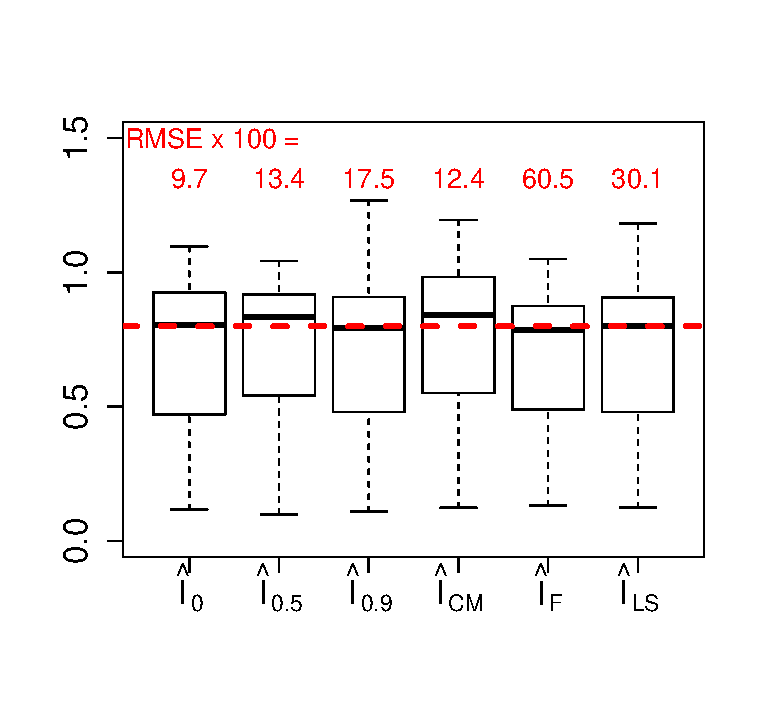
\includegraphics[scale = 0.5, clip = true, trim = 0 0.5in 0 0.5in]{../info_theory_sims/fig1.pdf}
\end{center}
Na\"{i}ve estimator performs best!  $\hat{I}_{LS}$ not effective.

Sampling distribution of $\hat{I}$ for \small{$\{p = 50$, $B = \frac{4}{\sqrt{50}} I_{50}$, $K = 20$, $r = 8000\}$.}

True parameter $I(X; Y) = 1.794$ \emph{(dashed line.)}
\begin{center}
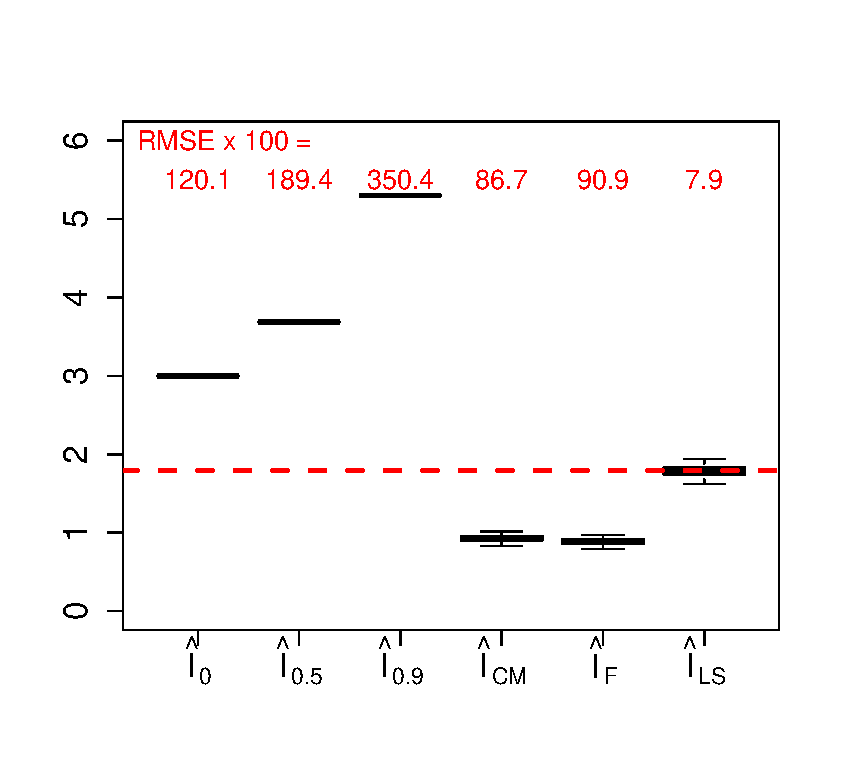
\includegraphics[scale = 0.5, clip = true, trim = 0 0.5in 0 0.5in]{../info_theory_sims/fig2.pdf}
\end{center}
Non-parametric methods extremely biased.

Estimation path of $\hat{I}_{LS}$ and $\hat{I}_\alpha$ as $n$ ranges from $10$ to $8000$.

\small{$\{p = 10$, $B = \frac{4}{\sqrt{10}} I_{10}$, $K = 20\}$.
True parameter $I(X; Y) = 1.322$ \emph{(dashed line.)}}

\begin{center}
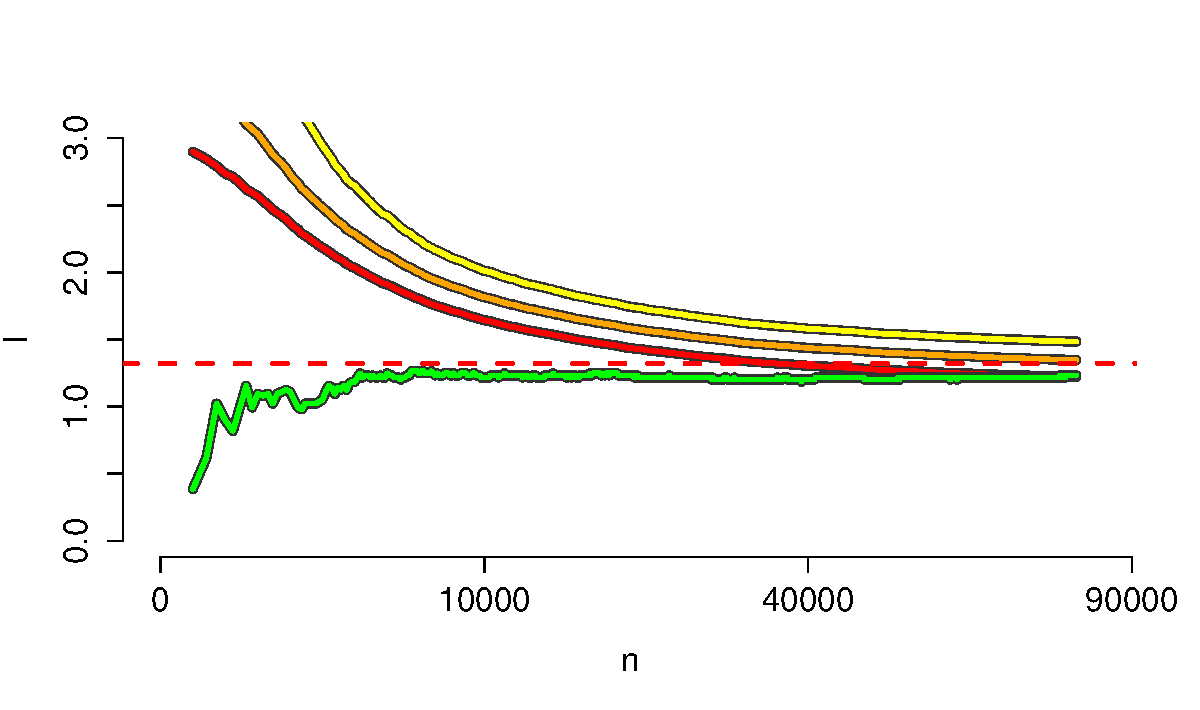
\includegraphics[scale = 0.4]{../info_theory_sims/fig3.pdf}
\end{center}

\begin{center}
\textbf{Estimated $\hat{I}$ vs true $I$.} 

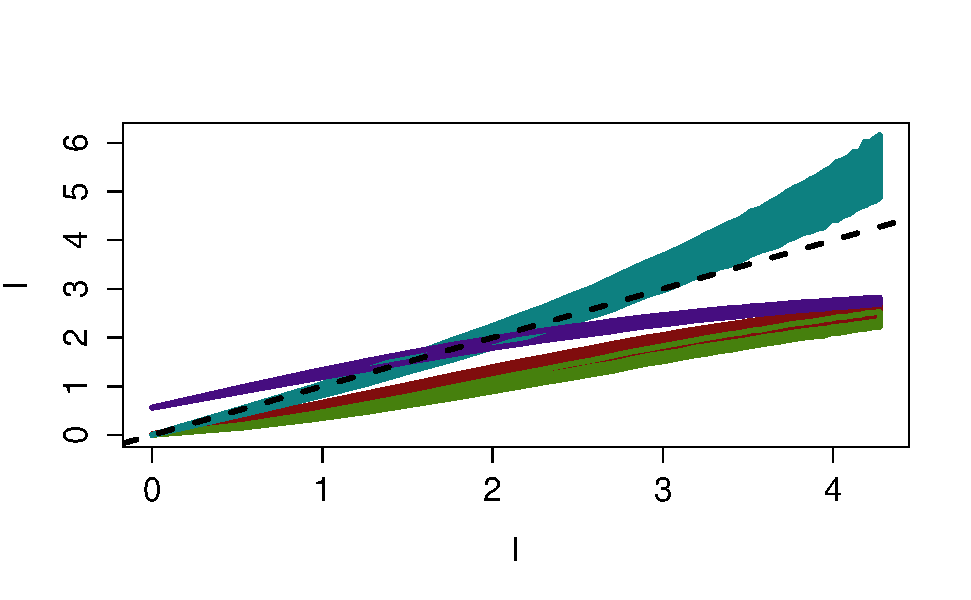
\includegraphics[scale = 0.5, clip=true, trim=0.4in 0.5in 0 0.5in]{../info_theory_sims/fig4.pdf}
\end{center}

Sampling distribution of $\hat{I}_{LS}$ for \small{$\{p = 10$, $B = \frac{4}{\sqrt{10}} I_{10}$, $N = 80000\}$,

and $K = \{5, 10, 15, 20, \hdots, 80\}$, $r = N/k$.}

True parameter $I(X; Y) = 1.322$ \emph{(dashed line.)}
\begin{center}
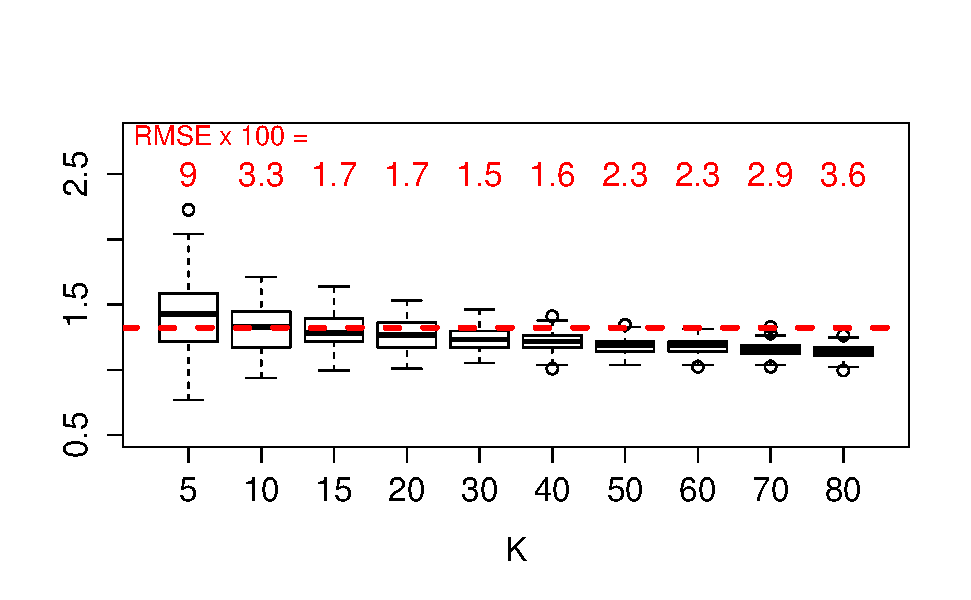
\includegraphics[scale = 0.6, clip = true, trim = 0 0.5in 0 0.5in]{../info_theory_sims/fig5a.pdf}
\end{center}

Decreasing variance as $K$ increases. Bias at large and small $K$.

$p = 20$ and $q = 40$, entries of $B$ are iid $N(0, 0.025)$.

$K=20$, $r = 8000$, true $I(X; Y) = 1.86$ \emph{(dashed line.)}

\begin{center}
\textbf{Sampling distribution of $\hat{I}$.}
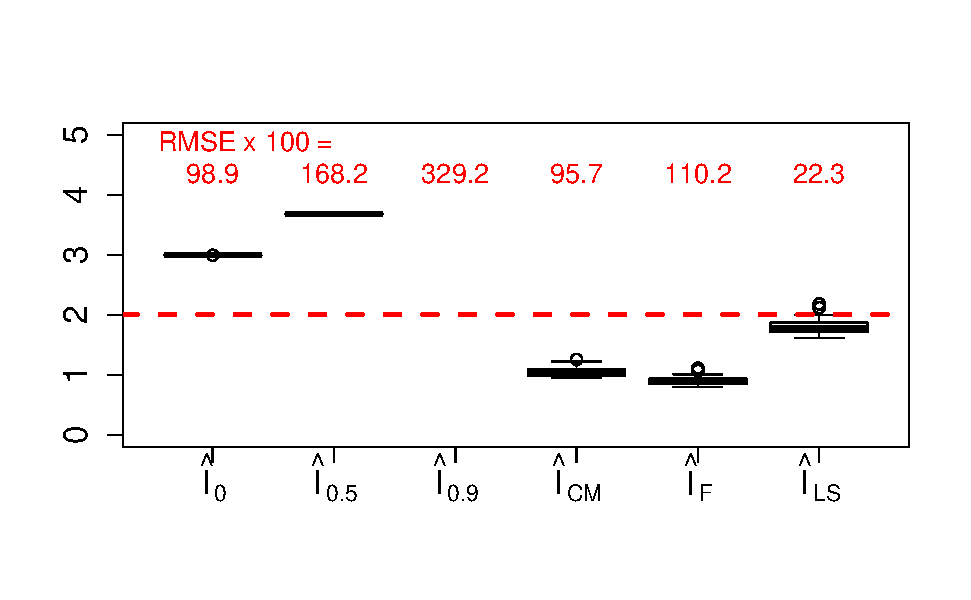
\includegraphics[scale = 0.6, clip = true, trim = 0 0.5in 0 0.5in]{../info_theory_sims/fig6.pdf}
\end{center}

\section{Conclusions}

\begin{itemize}
\item We derive a relationship between average Bayes error (ABE) and mutual
  information (MI), motivating a novel estimator $\hat{I}_{LS}$.
\item Theory based on high dimensional, low SNR limit,
where \[\text{ABE} \leftrightarrow \text{MI}.\]
\item In ideal settings for supervised learning, ABE can be estimated
  effectively and $\hat{I}_{LS}$ can recover MI at much lower sample
  sizes than nonparametric methods.
\item In simulations, $\hat{I}_{LS}$ works better than Fano's
  inequality or the confusion matrix approach.
\end{itemize}

\section{References}
\begin{itemize}
\item Cover and Thomas.  Elements of information theory.
\item Muirhead.  Aspects of multivariate statistical theory.
\item van der Vaart.  Asymptotic statistics.
\end{itemize}
\end{document}





